%&tex
% !TEX program = xelatex
% !TeX TS-program = xelatex
% !BIB TS-program = biber
% !TeX encoding = UTF-8
% !TeX spellcheck = en_US
% !TeX root = ../thesis.tex
%% ==============================
\section{Programmable Logic Controllers}
\label{sec:plc}
%% ==============================

 
\begin{figure}
    \centering
    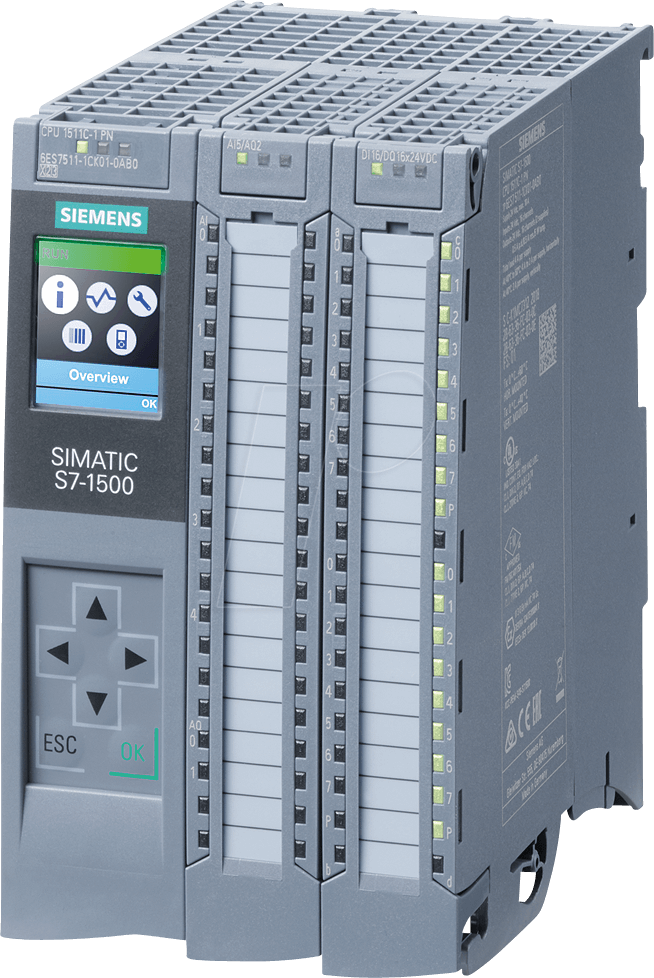
\includegraphics[width=0.5\textwidth]{Figures/simatic_s7-1500.png}
    \caption[Siemens SIMATIC S7-1500]{Siemens SIMATIC S7-1500~\acrshort{acn:plc}~\cite{Reichelt:2020}}
    \label{fig:simatic_s7}
\end{figure}

This section explains the basics of~\glspl{acn:plc} and their programming model.
They are a staple of industrial automation since the mid to late 1970's.
Major manufactures include Siemens, Rockwell Automation (Allen Bradley), Schneider Electric, Mitsubishi Electric, Omron, ABB, and General Electric~\cite{Businesswire:2016}.
Figure~\ref{fig:simatic_s7} shows an example of a modern Siemens mid range~\acrshort{acn:plc} with an attached power supply and a I/O module.

\subsection{General}

\begin{figure}
    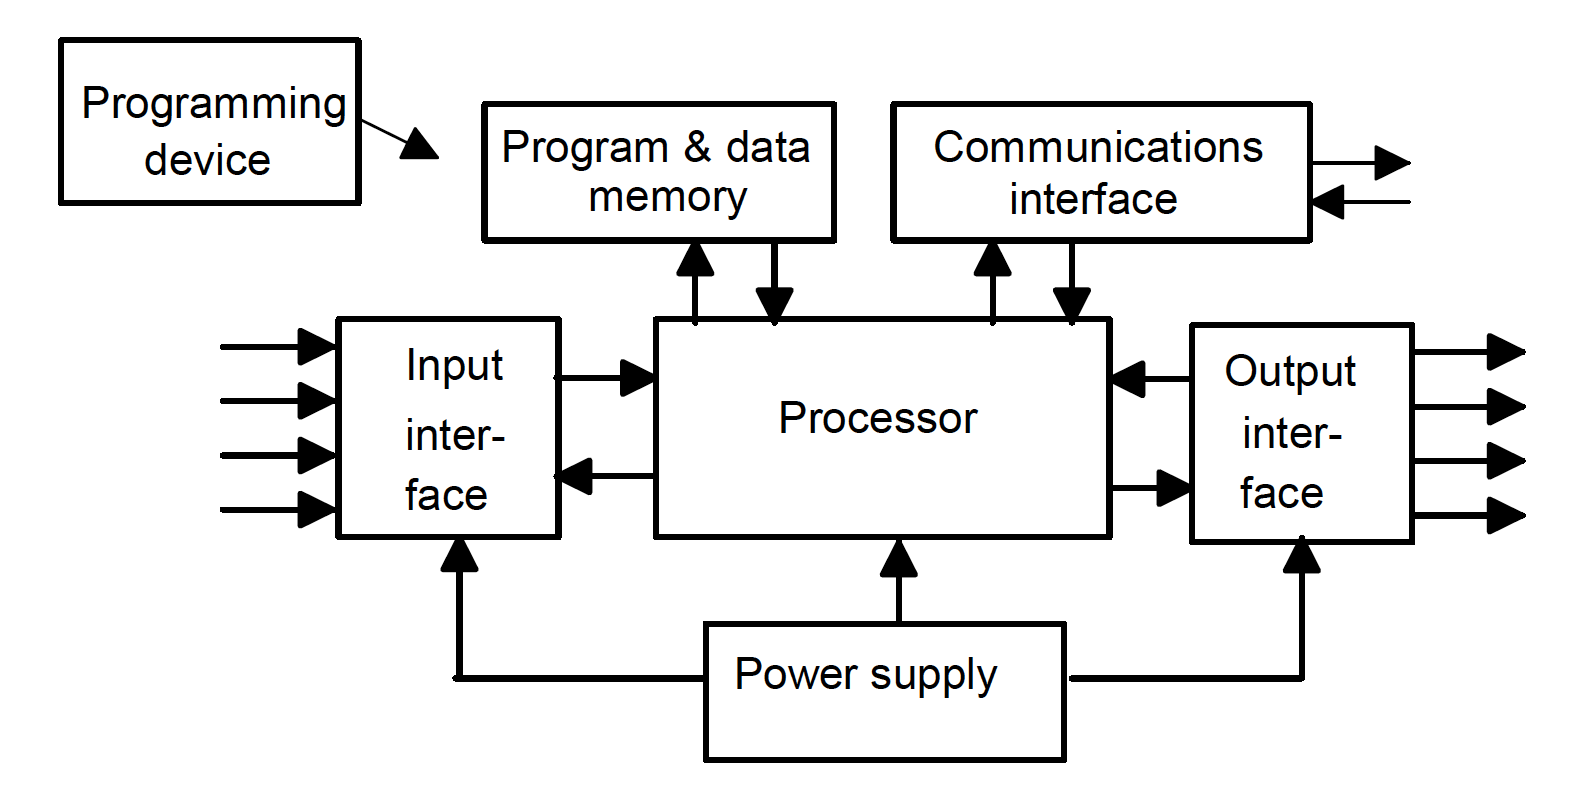
\includegraphics[width=\textwidth]{Figures/PLC_Architecture.png}
    \caption[PLC Architecture]{
       PLC Architecture~\cite[p.~4]{BOLTON200653}.
    The input and output interfaces are either digital or analog electrical signals.
    Memories are controlled by the OS on the PLC and are programmed with an external programming device.
    Additionally, PLC have a communications interface that allows it to communicate with other controllers or devices.}
    \label{fig:plc_architecture}
\end{figure}

A~\acrfull{acn:plc} is a controller that can be programmed via simple instructions to allow the easy processing of inputs and outputs~\cite[p.~4]{BOLTON200653}.
Figure~\ref{fig:plc_architecture} shows the basic components of a~\acrshort{acn:plc}.
\acrshort{acn:plc}s consist of input and output interfaces as well as a CPU that executes the current program on the inputs.
The program memory allows to change the programming of  the~\acrshort{acn:plc} without adapting any hardware components.
Additionally, the data memory can be used create persistent data for creating stateful programs.
Lastly~\acrshort{acn:plc} contain a communications interface that allows the communication with other controllers or a supervisor software.
This can for example also be used to send sensor data to a central database or implement a self-management system.

A major advantage of~\acrshort{acn:plc} is that they allow for a modular design~\cite[p.~12]{BOLTON200653}, as seen with the Siemens~\acrshort{acn:plc} in figure~\ref{fig:simatic_s7}.
They are commonly assembled in a rack which allow to combine multiple modules to create a flexible configuration.
Additional hardware components, such as memory, processors, communication or I/O modules can be added with minimal effort.
This allows for standardized yet individually configurable hardware setups.
Many vendors also provide non modular single-box solutions.

Another difference between a~\acrshort{acn:plc} and a regular micro-controller is the execution semantic of a program.
\acrshort{acn:plc} programs are executed in repeating cycles.
Each cycle consists of three distinct phases: reading of input values into the~\acrshort{acn:ram}, execution of the program and the writing of the output variables from the~\acrshort{acn:ram}~\cite[p.~75]{BOLTON200653}.
These cycles are executed continuously during runtime if a cycle is finished a new one starts.
The time it takes to execute a single cycle is called the cycle time.
This time depends on the processing power of the hardware, and the program complexity.
Because of this execution semantic, changes to the input during a cycle are not registered until the beginning of the next cycle, and new output values are not present until the end of the current cycle.
Therefore, input values must be present for at least the cycle time to ensure they are read.
This provides a deterministic behavior of the PLC and allows for real-time capability.

\subsection{Programming with IEC 61131-3 Languages}

\acrshort{acn:plc}s are programmed with one of the five languages defined in the~\textit{IEC 61131-3}~\cite{Plcopen:61131-3} standard.
These languages are designed to provide a safe and well-defined way of handling the inputs and outputs of the controller.
Additionally, these languages are intended to be used by an automation or electrical engineer rather than an experienced programmer.
As a result, all these languages have reduced complexity compared to a language like C.
This subsection gives more details on the two most common languages used for~\acrshort{acn:plc} programming,~\acrfull{acn:ST} and the~\acrfull{acn:LD}.

In general, the languages have access to the input data read from the inputs and are expected to write output values to the outputs.
They also have access to the memory allowing to read data from previous cycles or write data for future cycles.
% Requried so that structured text is on a new page.
\\
\subsubsection{Structured Text}
\lstset{language=Pascal}
\begin{lstlisting}[caption={
Example of~\gls{acn:ST} code for controlling a conveyor belt and a drill.},label=lst:ex:st]
// PLC configuration
CONFIGURATION DefaultCfg
	VAR_GLOBAL
		b_Belt_Wants_ON  : BOOL;

		// Digital input of the PLC (Address 0.0).
		Position_A_Free     AT %IX0.0:BOOL;
		// Digital input of the PLC (Address 0.1).
		Position_B_Free     AT %IX0.1:BOOL;

		// Digital output of the PLC (Address 0.0). (Coil)
		Drill_ON            AT %QX0.0:BOOL;
		// Digital output of the PLC (Address 0.1). (Coil)
		Belt_ON             AT %QX0.1:BOOL;
	END_VAR

	// Schedule the main program to be executed every 20 ms
	TASK Tick(INTERVAL := t#20ms);

	PROGRAM Main WITH Tick : Drill_Belt_Control;
END_CONFIGURATION

// Actual Program
PROGRAM Drill_Belt_Control          
	VAR_EXTERNAL
		Position_A_Free     : BOOL;
		Position_B_Free     : BOOL;
		Drill_ON            : BOOL;
		Belt_ON             : BOOL;
	END_VAR

	IF NOT Position_A_Free THEN
		b_Belt_Wants_ON := False;
		Drill_ON := True;
	ENDIF;

	IF Position_A_Free AND NOT Position_B_Free THEN
		b_Belt_Wants_ON := True;
	ENDIF;

	IF NOT Drill_ON AND b_Belt_Wants_ON THEN
		Belt_ON := True;
	ENDIF;
END_PROGRAM
\end{lstlisting}

\acrfull{acn:ST} is one of the two textual languages defined in the~\textit{IEC 61131-3} standard.
It follows a PASCAL like syntax, allowing for a higher level of abstraction compared to the other languages for~\acrshort{acn:plc} programming.

Listing~\ref{lst:ex:st} shows an example of~\acrshort{acn:ST} code for a~\acrshort{acn:plc}.
This example models a setup with two proximity sensors, to detect if an object is occupying a place on the conveyor belt, and two motors, one to drive the belt and one to activate a drill.
You can see that~\acrshort{acn:ST} allows to handle programs like high level languages such as C.
The first configuration part defines a mapping of variables to physical address, defines the cycle time and the main program.
Additionally, the~\textit{b\_Belt\_Wants\_ON} variable that is stored in the memory and not mapped to an in-/output is defined.
The second part defines the main program.
Here you can see that the input and output variables can be used in the same way as regular variables.
As mentioned before the initial values for the variables will be read from the physical inputs before the execution, and the values of the output variables at the end of the execution are written to the physical outputs.

This shows that programming in~\acrshort{acn:ST} is similar to programming in regular PASCAL.
Its compact structure and high-level approach allow the engineer to write advanced programs easier.
\acrshort{acn:ST} supports advanced control structures like~\textit{FOR} or~\textit{WHILE} loops making it easier to implement complex algorithms compared to the other PLC languages. 
To further manage complexity, it supports function declaration.
This makes~\acrshort{acn:ST} the best candidate function for implementing complex functionality in a~\acrshort{acn:plc}.
The real-time functionality is realized via the pre-defined cycle time.
\acrshort{acn:plc} environment allow to simulate and statically analyze~\acrshort{acn:ST} code to ensure the cycle times are met.

\subsubsection{Ladder Diagram}

The most used language for~\acrshort{acn:plc} programming is~\acrfull{acn:LD}.
It resembles the definition of an electrical circuit by graphically combining logical blocks to implement functionality.
Figure~\ref{fig:drill:ld} shows the same functionality implemented in~\acrshort{acn:ST} in listing~\ref{lst:ex:st} implemented in~\acrshort{acn:LD}.

\acrshort{acn:LD} assumes a value of 1 on the left vertical line and a ground connection on the right line.
On the horizontal lines, logical blocks related to input, output or memory variables can be added to create logical functions.
In the example the circle blocks on the right symbolize the writing to the memory and the symbols on the left are read accesses and logical operations on variables in the memory.

This language is for historical importance as it was the first commonly used programming language for~\acrshort{acn:plc} programming.
Its structure is like the one used for programming traditional electrical relays.

\begin{figure}[h]
	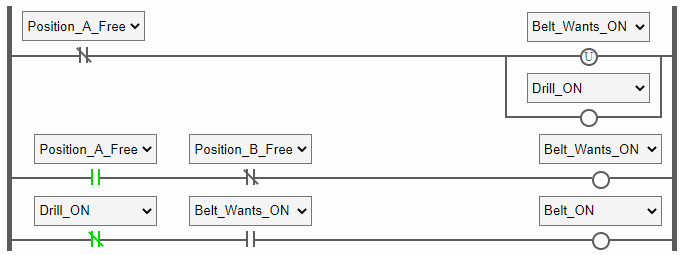
\includegraphics[width=\textwidth]{Figures/belt_drill_ld.png}
	\caption[Drill and Belt controller example in Ladder Diagram]{Drill and Belt controller example in Ladder Diagram}
	\label{fig:drill:ld}
\end{figure}